% !TeX root = ../main.tex
% Add the above to each chapter to make compiling the PDF easier in some editors.

\chapter{Implementation}\label{chapter:Implementation}
The subsequent chapter is going to give a detailed view of how the methods described in section \ref{chapter:Concept}, were implemented. Moreover, possible problems regarding the process are listed. 
As I took the Android-application described in passage \ref{chapter:Integration into existing App} as a basis, there is no reasonable alternative to further developing the app with Android Studio.

\section{Native Development Kit}
The Android NDK is a toolset that lets you implement parts of your app in native code, using languages such as C and C++. For certain types of apps, this can help you reuse code libraries written in those languages \cite{androidndk}. Moreover employing the Native Development Kit to your Java code can increase the performance of the application significantly  \cite{ndkspeed}. I anticipated using the Native Kit might have a bigger workload, than Android's classic SDK, but I thought this to be alright if the performance was superiorly compared to the approach written in Java. \newline
The first part, dealing with the detection of Speed Signs, doing image processing with OpenCV,  was relatively simple in C++, compared to the mammoth task of building Tensorflow from source, loading a model and integrating everything into the actual app. It actually was so time-consuming, I did not think I could manage to make it work on schedule. A lack of supporting features like Code Completion in Android Studio, poor documentation from Tensorflow (at least for average developers) paired with proportionally sparse discussion board entries like "Stack Overflow", that often referenced different versions, led me to the turning point, where I gave up using the NDK for the SDK. In total, this excursion cost me about one to two weeks of my time, reserved for the implementation.  

\section{Extracting Speed Sign Candidates}
I implemented the algorithm in three languages: C++, Java and Python, every language serving different purposes. C++ and Java versions were necessary to operate for the application, first, one running the Native approach, the second for the "standard" version. The last program written in Python was utilized for extracting data from images collected from Google image search, running on my PC, in order to get training data to feed my Neural Network model (more about this topic later on). Nevertheless, apart from syntactical differences, every program basically does the same operations. For the sake of simplicity, I am only going to present the python variation, as it is probably the easiest to read. Every step of image processing in every language has been done with the OpenCV library. \newline
After reading the image, changing the colour space from RGB/BGR to HSL/HSV is optional, but a reasonable step, because in the RGB/BGR space, all three Values of red, green and blue are correlated when it comes to changes in brightness \cite{imagesegmentation}. Unlike that, HSL/HSV holds lightness or the value of brightness in a separate variable, which can lead to better results with respect to filtering colours under difficult lighting conditions. In the following, we are going to stick to the HSV space, even though both work almost analogical, they differentiate each other from the arrangement of brightness. \newline
Nevertheless filtering red pixels from our preferred colourspace works slightly different than just excerpting the Red channel of an image, as you would using RGB:
\begin{figure}[H]
	\minipage{\textwidth}
	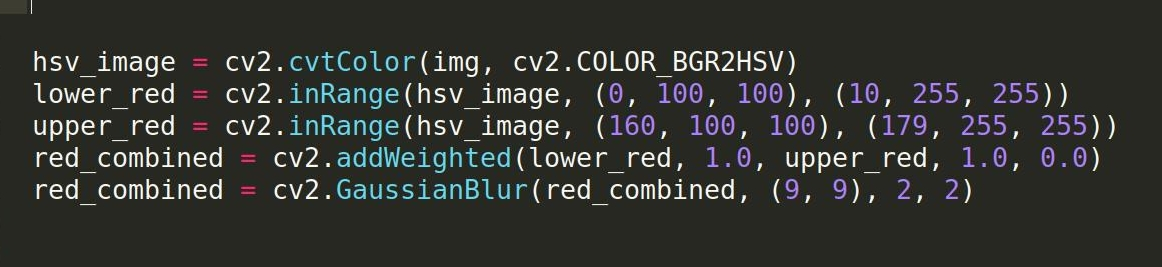
\includegraphics[width=\linewidth]{images/filterredimage.jpg}
	\caption{Python code for extracting red pixels}\label{fig:filter_red_code}
	\endminipage\hfill
\end{figure}
At first you extract ranges of HSV values, that are considered to be red. This is done in two slices, for the upper range (Figure: \ref{fig:lower_red}), and one for the lower (Figure: \ref{fig:upper_red}). After these two slices are combined into one single binary image (Figure: \ref{fig:combined}), the Gaussian Blur filter is executed (Figure: \ref{fig:combined_blurred}) on the image, to prepare it for the Circle Hough transform, in order to avoid false positive circles.\newline
 
\begin{figure}[H]
	\minipage{\textwidth}
	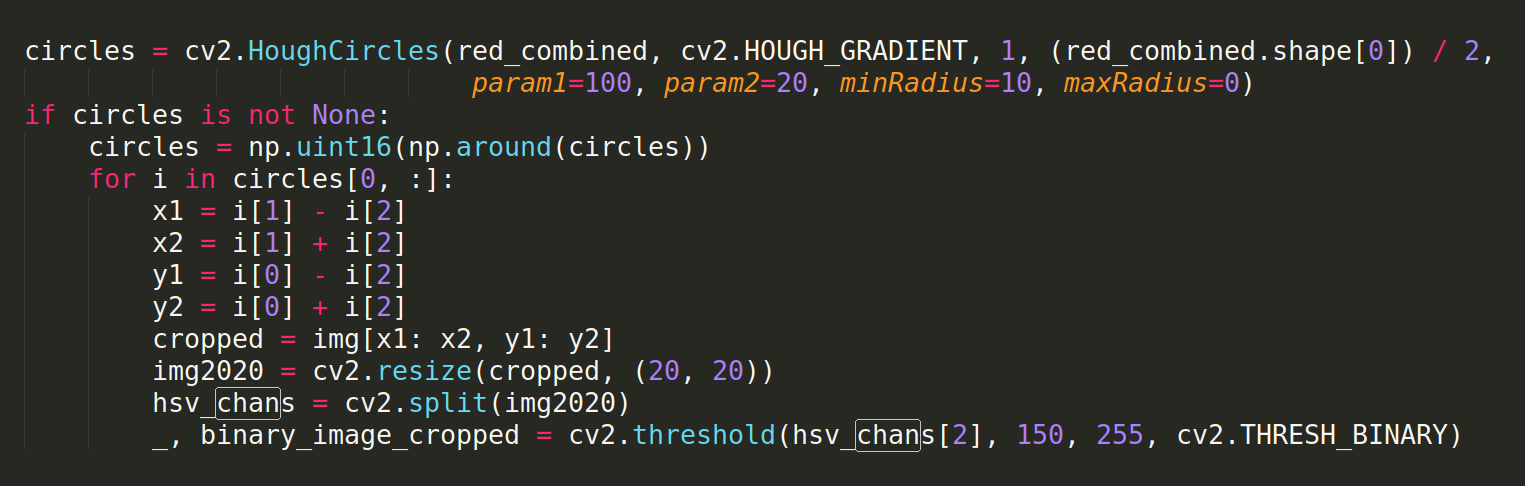
\includegraphics[width=\linewidth]{images/detectioncode.png}
	\caption{Code for performing Circle Hough Transform}\label{fig:detection_code}
	\endminipage\hfill
\end{figure}
When executing the HoughCircles Function \cite{houghcircles}, the result is passed to the circles variable, this function returns all found circles, described with an array of [x-coordinate, y-coordinate, radius],  after checking, whether any circles were found, we only have to round these values to integer and loop over the array containing every triplet. \newline
In order to crop our input image, the x- and y- coordinates of the cropping window are calculated, this window can be described by the coordinates of two edges. After actually cropping the image we resize this section to our desired 20 by 20 pixels format (Figure: \ref{fig:2020}). Then we convert this sub picture from coloured to binary format (Figure: \ref{fig:2020bin}). Now the image is actually ready, to be passed to the Neural Network. It should be noted, there can be multiple candidates in one image that need to be passed further.   

\begin{figure}[H]
	\minipage[t]{0.33\textwidth}%
	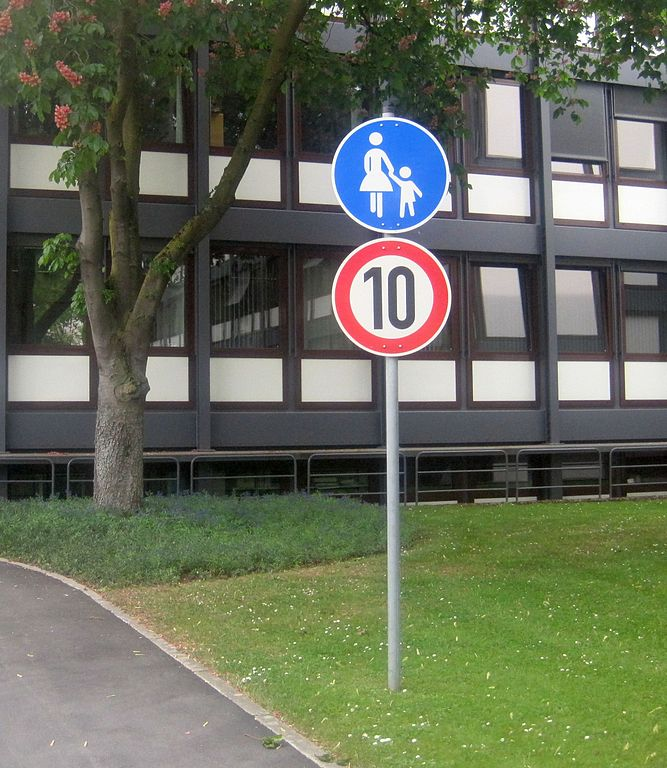
\includegraphics[width=\linewidth]{images/101.jpg}
	\caption{Original Image}\label{fig:original_image}
	\endminipage\hfill
	\minipage[t]{0.33\textwidth}
	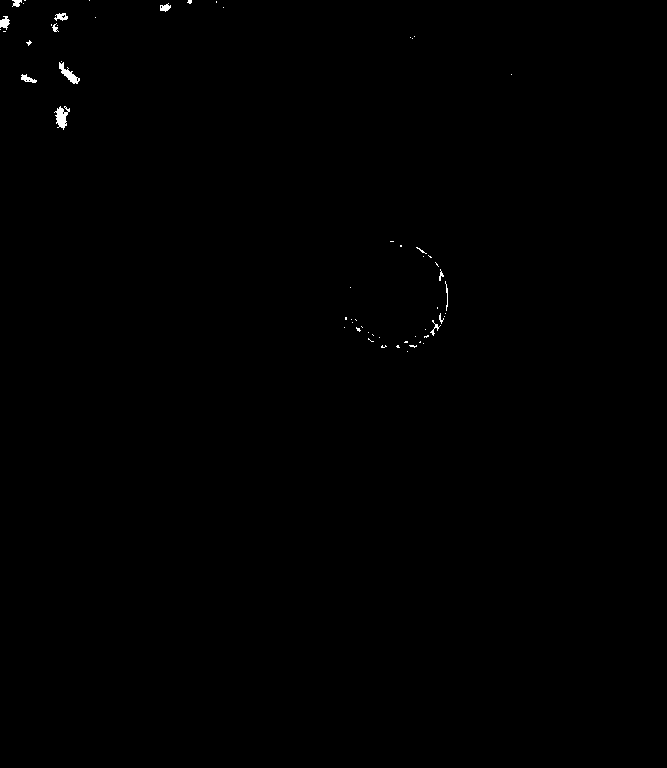
\includegraphics[width=\linewidth]{images/lowerred.png}
	\caption{Lower red hue pixels}\label{fig:lower_red}
	\endminipage\hfill
	\minipage[t]{0.33\textwidth}%
	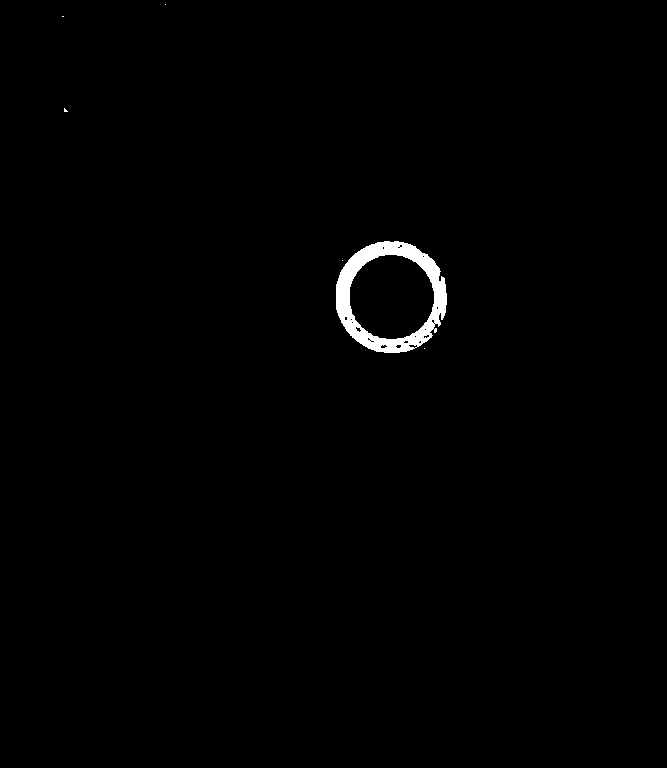
\includegraphics[width=\linewidth]{images/upperred.png}
	\caption{Upper red hue pixels}\label{fig:upper_red}
	\endminipage\hfill
	\newline
	\newline
	\minipage[t]{0.33\textwidth}
	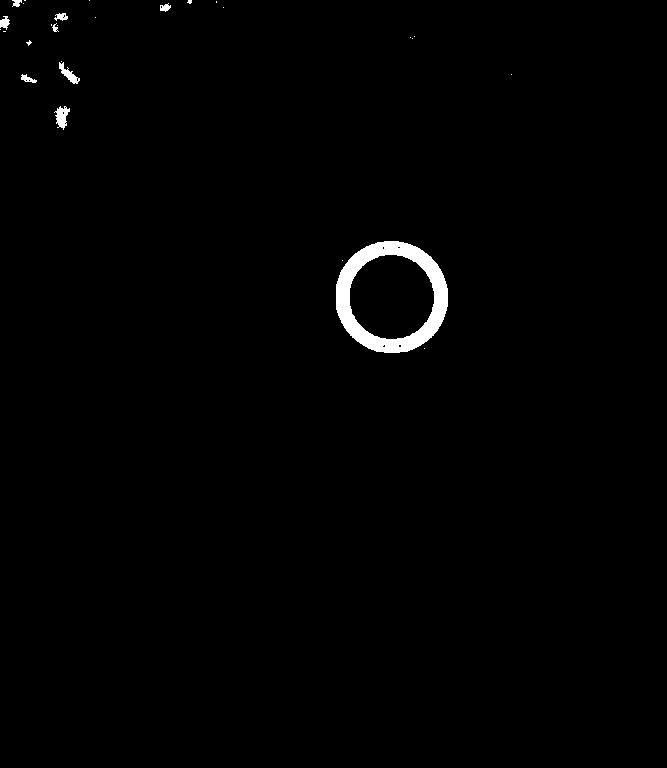
\includegraphics[width=\linewidth]{images/redcombined1.png}
	\caption{Upper and lower pixels combined}\label{fig:combined}
	\endminipage\hfill
	\minipage[t]{0.33\textwidth}
	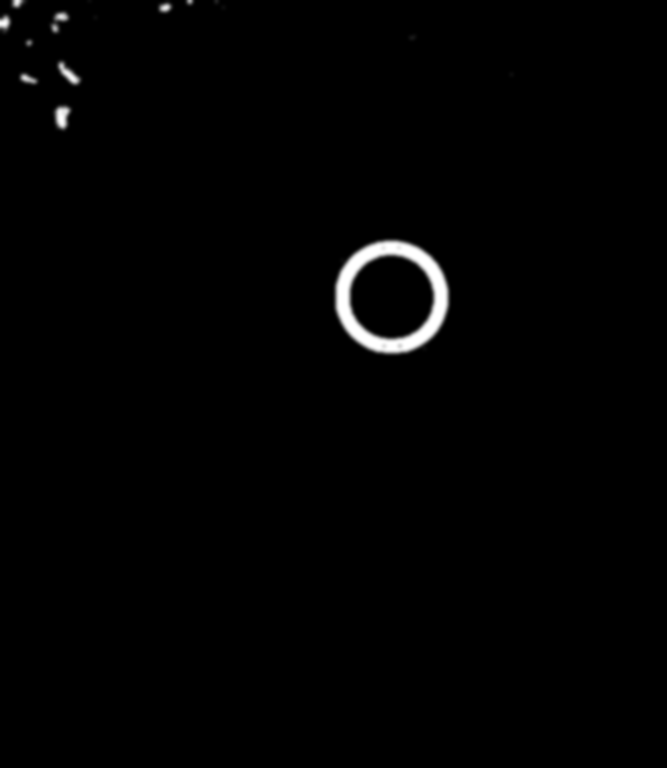
\includegraphics[width=\linewidth]{images/redcombined2.png}
	\caption{Gaussian Blurred}\label{fig:combined_blurred}
	\endminipage\hfill
	\minipage[t]{0.33\textwidth}
	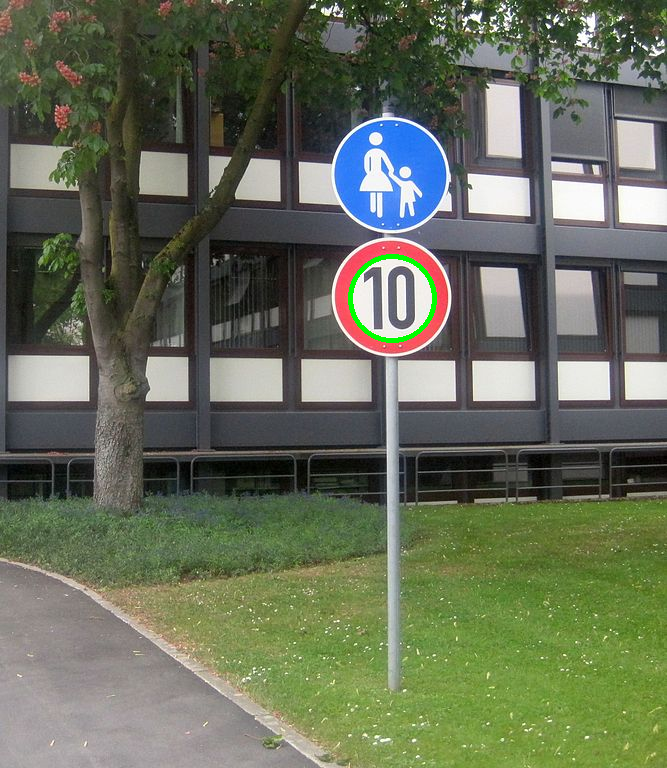
\includegraphics[width=\linewidth]{images/detectedcirclescircle.png}
	\caption{Marked circle in original image}\label{fig:detectedcircles}
	\endminipage
	
\end{figure}

\begin{figure}[H]
	\minipage[t]{0.49\textwidth}%
	
\includegraphics[width=\linewidth]{images/2020.png}
	\caption{Cropped image}\label{fig:2020}
	\endminipage\hfill
	\minipage[t]{0.49\textwidth}%
	
\includegraphics[width=\linewidth]{images/binaryimg.png}
	\caption{Cropped and converted image}\label{fig:2020bin}
	\endminipage\hfill
	\newline
	
\end{figure}


\begin{figure}[H]
	\centering
	\minipage{0.5\textwidth}
	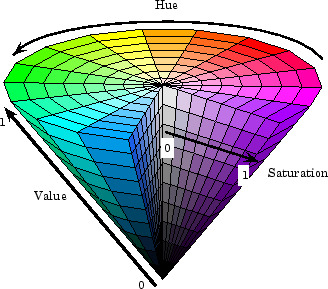
\includegraphics[width=\linewidth]{images/hsv.jpg}
	\caption{HSV colourspace \cite{hsv}}\label{fig:hsv}
	\endminipage\hfill
\end{figure}



\section{Neural Net Classification}
Hypothetically speaking, we only need to put this image into a tensor, feed it into our model and get the result back. Getting to this point there needs to be done some work, regarding our Neural Network though.  
\subsection{Building Neural Network with Tensorflow}
TensorFlow™ is an open source software library for numerical computation using data flow graphs. Nodes in the graph represent mathematical operations, while the graph edges represent the multidimensional data arrays (tensors) communicated between them. \cite{tensorflow} When it comes to building models on a PC, you could use Tensorflow's C++, Go, Java or Python API, although the core is programmed in C++ \cite{tensorflowcore}. I decided to use the Python API, because again I thought this language to be the easiest choice. \newline
\begin{figure}[H]
	\centering
	\minipage{\textwidth}
	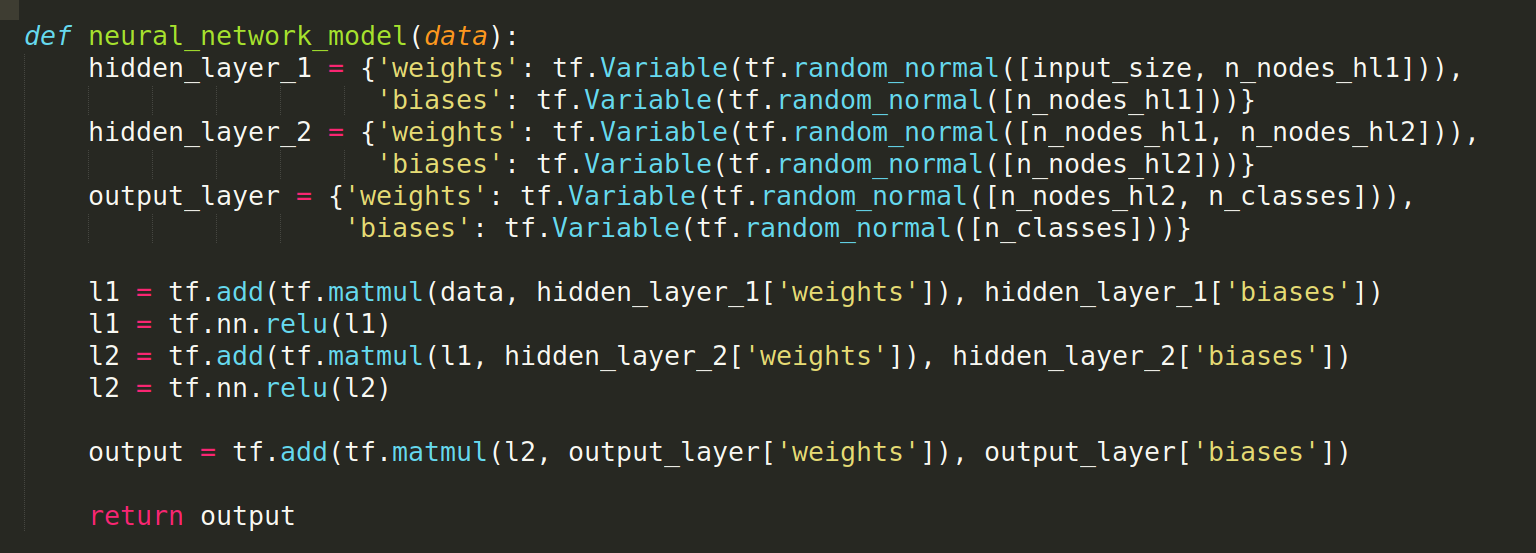
\includegraphics[width=\linewidth]{images/neuralnetmodelcode.png}
	\caption{Neural Net Model in Python}\label{fig:NNmodelPyth}
	\endminipage\hfill
\end{figure}

Obviously, the "data" parameter, given to the neural\_network\_model represents our input tensor, thus it holds every pixel provided by the image. The dictionaries "hidden\_layer\_1", "hidden\_layer\_2" and "output\_layer" hold the weights and biases of the incoming edges, they are all initialized with random values before the training phase. The "tf.add" and "tf.mul" adds, respectively multiplies two tensors. The variables "l1" and "l2" each have two initialization steps, in the first, preceding nodes are multiplied with the corresponding weights and added to it's biases. The second part calls "tf.nn.relu", which is just the activation function used for this network. The "output" variable finally holds and returns the final output tensor. 
